\documentclass[a4paper,10pt]{article}
\usepackage[utf8]{inputenc}
\usepackage{graphicx}
%opening
\title{TH7}
\author{R.P.Clark}
\begin{document}
\maketitle
\begin{abstract}
This leaflet describes the TH7 generic thermocouple reader pi-hat/PCB for the raspberry pi.
\end{abstract}

\begin{figure}[ht]
 \centering
 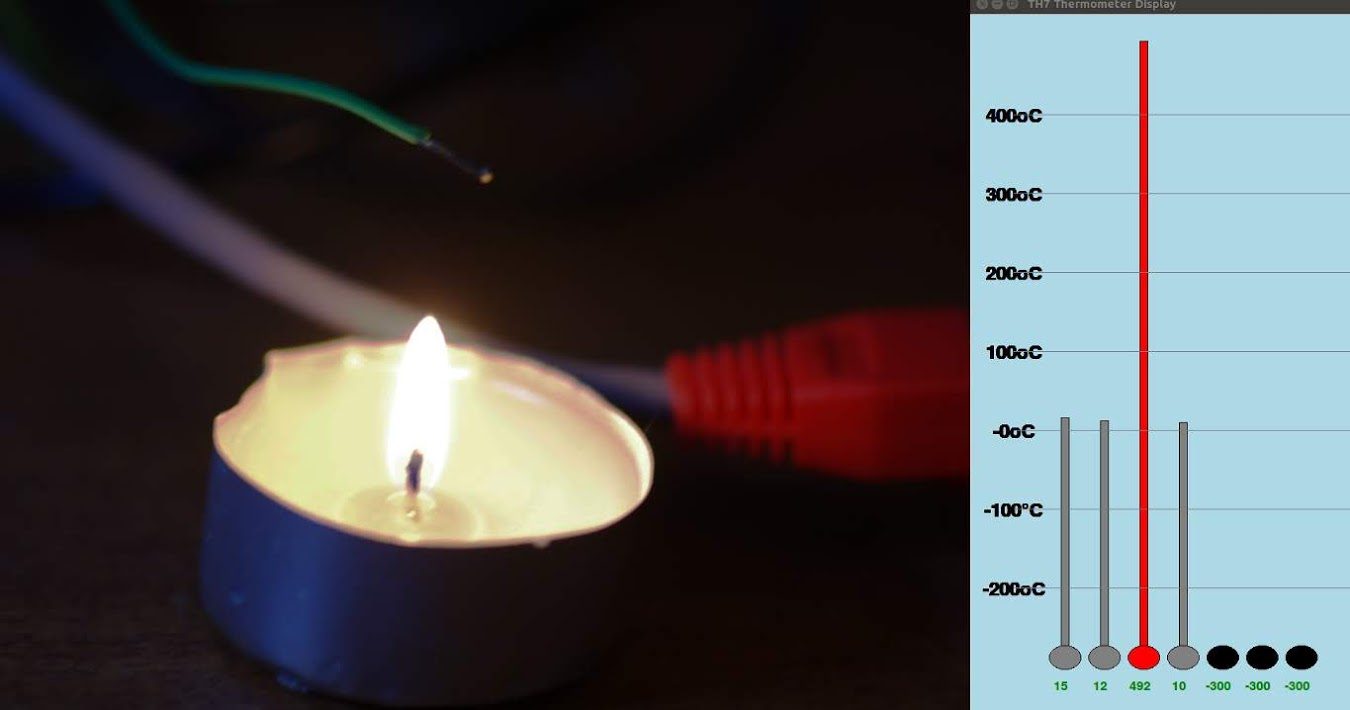
\includegraphics[width=300pt]{TH7_tea_light.JPG}
 % TH7_tea_light.JPG: 0x0 pixel, 300dpi, 0.00x0.00 cm, bb=
 \caption{Thermocouple over a tea light flame at circa ${500}^{\circ} C$.}
 \label{fig:pi}
\end{figure}

\section{TH7 description}
The TH7 is a raspbery pi hat (see figure~\ref{fig:th7} with on board PCB temperature measurement that
provides seven thermocouple inputs.
Uncalibrated this gives a typical accuracy of $\pm$ ${2}^{\circ} C$.
It also provides two user programmable LEDS and displays the supply voltage to the pi.

It ius a generic thermcouple reader, and therefore should work with any thermocouple.
Software support has been written for the `k' type only currently.

The TH7 offers:
\begin{itemize}
 \item Full cold junction compensation
 \item Loss of/disconnection of thermocouple detection
 \item Seven inputs
 \item Uses the rasberry pi standard python SPI interface
 \item Python coding examples (https://github.com/robin48gx/TH7).
\end{itemize} 

\section{Instructions}

Connect the thermocouples using the hital~tech connectors and ensdure the wires make contact with the 
connector metal clams (see figure~\ref{fig:con}.
Always apply insulation to the thermocouples (i.e. do not ground them).
Epoxy resin is often useful for gluing thermcouples to devices under long term temperature test.

\begin{figure}[h]
 \centering
 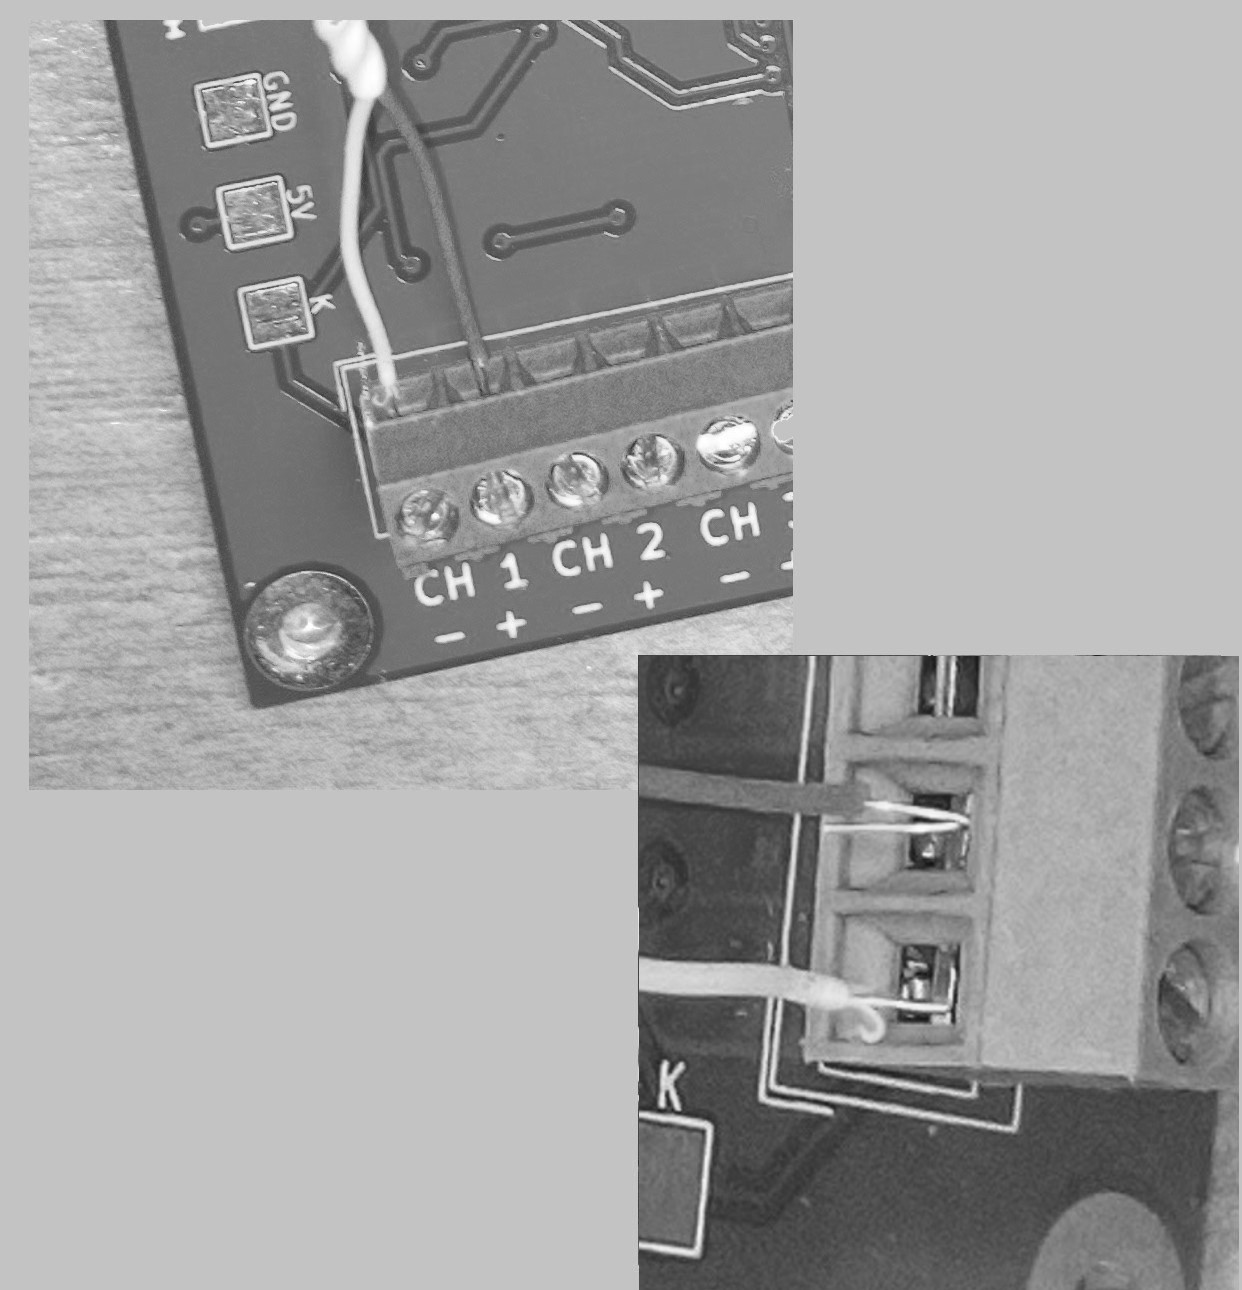
\includegraphics[width=200pt]{./wiring.JPG}
 % wiring.JPG: 0x0 pixel, 300dpi, 0.00x0.00 cm, bb=
 \caption{Wiring European standard `k' type thermocouples Wiring. The green is plus and the green and white is minus. Other countries may use different colour schemes. 
 If the thermoucouple is inserted with incorrect polarity temperature will be seen to go down when heat is applied to it.}
 \label{fig:con}
\end{figure}

\begin{figure}[h]
 \centering
 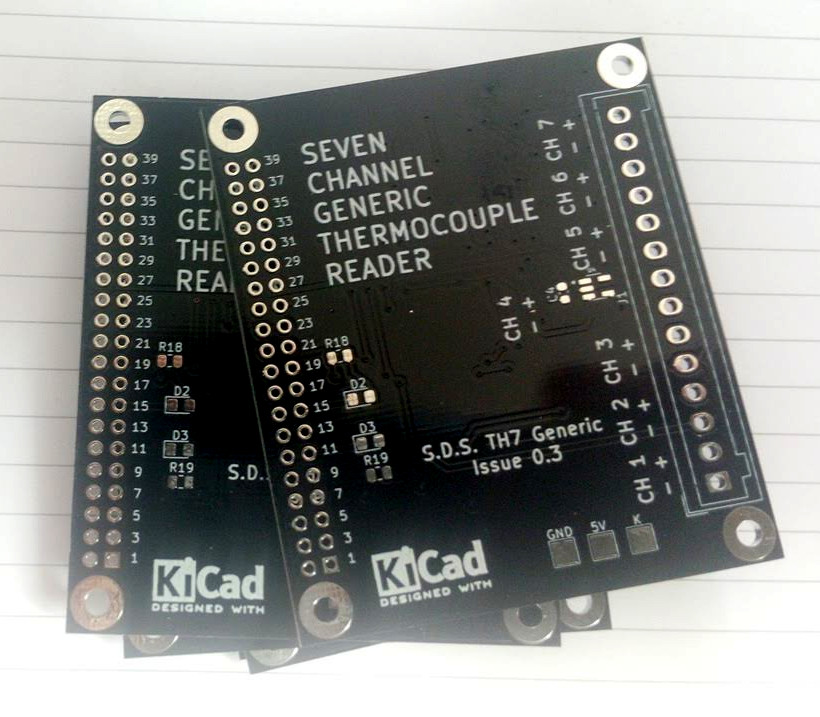
\includegraphics[width=156pt]{./TH7_0p3.jpg}
 % TH7_0p3.jpg: 0x0 pixel, 300dpi, 0.00x0.00 cm, bb=
 \caption{TH7 thermocouple interface PCB/pi~Hat}
 \label{fig:th7}
\end{figure}



\end{document}
